\documentclass[12pt,a4paper]{report} % Classe report con dimensioni standard
\usepackage[utf8]{inputenc} % Supporto per i caratteri UTF-8
\usepackage[T1]{fontenc} % Migliora la gestione dei font
\usepackage{graphicx} % Per includere immagini
\usepackage{amsmath} % Supporto per formule matematiche
\usepackage{geometry} % Per personalizzare i margini
\geometry{a4paper, margin=1in} % Margini di 1 pollice su tutto il foglio
\usepackage{setspace} % Per regolare l'interlinea
\setstretch{1.5} % Imposta interlinea a 1.5
\usepackage{hyperref} % Per collegamenti cliccabili
\usepackage{fancyhdr} % Per intestazioni e piè di pagina personalizzati
\pagestyle{fancy} % Attiva intestazioni e piè di pagina
\fancyhead[L]{SentAI} % Intestazione a sinistra
\fancyhead[R]{Giovanni Paolo Chierchia} % Intestazione a destra
\fancyfoot[C]{\thepage} % Numero di pagina centrato
\usepackage{float}
\usepackage[utf8]{inputenc}

%Formattazione codice
\usepackage{minted}
\setminted{
    style=trac,
    linenos,
    breaklines,
    tabsize=4,
}

% Evitare vedove e orfane
\clubpenalty=10000  % Evita le orfane
\widowpenalty=10000 % Evita le vedove
\displaywidowpenalty=10000 % Evita le vedove nei display math

\title{SentAI}
\author{Giovanni Paolo Chierchia}
\date{\today}

\begin{document}

% Pagina di copertina personalizzata
\begin{titlepage}
    \centering
    
\includegraphics[width=\textwidth]{immagini/SentAI-Logo.png}\\[1cm] % Logo del progetto
    {\Huge \textbf{SentAI}}\\[1cm]
    {\Large Sentiment analysis di commenti social}\\[1cm]
    \href{https://github.com/Giop378/SentAI}{\texttt{GitHub Repository}}\\[1cm]
    \textit{Progetto di Fondamenti Di Intelligenza Artificiale}\\
    \textit{Università di Salerno}\\[2cm]
    \textbf{Giovanni Paolo Chierchia [0512117783]}\\[0.5cm]
    \textbf{Prof. Fabio Palomba}\\[0.5cm]
    \textit{Febbraio 2025}
\end{titlepage}

\tableofcontents % Genera automaticamente l'indice

\chapter{Introduzione}
Negli ultimi decenni, l’avvento dei social media ha rivoluzionato la comunicazione, permettendo a milioni di utenti di esprimere opinioni e condividere esperienze in tempo reale. Questa nuova realtà ha generato una mole immensa di dati testuali, rendendo necessarie tecniche automatizzate per analizzarli.
La \textbf{sentiment analysis }si propone di identificare e classificare le emozioni espresse nei commenti online, distinguendo tra sentimenti positivi e negativi. Le aziende sfruttano questa tecnologia per monitorare la propria reputazione, personalizzare le strategie di marketing, condurre ricerche di mercato e migliorare il servizio clienti, trasformando dati grezzi in informazioni strategiche per decisioni più informate.

\chapter{Definizione del problema}
Essendo un problema in cui abbiamo bisogno di etichettare le nuove istanze che verranno date al Modello, e i dati stessi di traning sono anche essi etichettati, si può dedurre che questo è un problema di apprendimento supervisionato discreto e più nello specifico di \textbf{classificazione binaria}.
\section{Obiettivi}
L’obiettivo di questo progetto è sviluppare un sistema in grado di analizzare \textbf{brevi testi inseriti dall’utente} (tweet, post o semplici frasi), classificandoli come positivi o negativi. Per farlo, verrà scelto un classificatore tra  \textbf{Naive Bayes} e \textbf{Logistic Regression}.
Il sistema sarà addestrato su una parte di un dataset di tweet, scelto perché \textbf{già etichettato}, ampio (\textbf{1,6 milioni di esempi}) e rappresentativo del linguaggio informale dei social media. I tweet spesso contengono \textbf{errori di battitura, slang, abbreviazioni, emoji testuali, caratteri speciali, link URL, menzioni e hashtag}, elementi utili per addestrare un modello capace di gestire testi brevi e rumorosi . Inoltre, un dataset basato sui social media garantisce \textbf{maggiore adattabilità} ad altri contesti reali, come post e frasi. Verrà poi testato su testi brevi di varia natura per valutarne la generalizzazione. 
Sarà inoltre realizzata una semplice \textbf{interfaccia grafica} che permetterà all’utente di inserire un testo e ottenere immediatamente il risultato. L’obiettivo finale è creare un’applicazione semplice e intuitiva, capace di fornire risultati in modo rapido.
\section{Specifica P.E.A.S.}
L'ambiente viene descritto tramite la formulazione P.E.A.S.
\subsection{Performance}
L'agente viene valutato in base a metriche di classificazione come \textbf{accuracy}, \textbf{precision} e \textbf{recall} oltre all'analisi della \textbf{matrice di confusione }per individuare errori di classificazione. Il tempo di risposta massimo dal click del bottone sull'interfaccia grafica deve essere di 5 secondi.
\subsection{Environment}
Il classificatore opera nell’ambiente dei social media, dove i post sono testi brevi che spesso contengono slang, emoticon, abbreviazioni e rumore informativo. L’ambiente frasi o post raccolti dai social, sia dati contenuti nel dataset \href{https://www.kaggle.com/datasets/kazanova/sentiment140}{\textbf{Sentiment140}}, contenente tweet etichettati come positivi o negativi. 
\subsection{Actuators}
L'agente agisce sull'ambiente assegnando un'etichetta di sentiment (positivo o negativo) ai testi analizzati.
\subsection{Sensors}
L'agente percepisce l'ambiente tramite il testo in ingresso, ricevuto attraverso una finestra di input.

\section{Caratteristiche dell'ambiente}
\begin{itemize}
    \item \textbf{Parzialmente osservabile}: Il modello ha accesso solo ai dati testuali disponibili nei tweet, ma non a informazioni contestuali come il tono della voce, il sarcasmo o il significato implicito dietro le parole.
\end{itemize}
\begin{itemize}
    \item \textbf{Stocastico}: Il sentiment di un tweet non è determ+inistico, poiché parole simili possono avere significati diversi in base al contesto e all'intenzione dell'autore.
\end{itemize}
\begin{itemize}
    \item \textbf{Episodico}: L'analisi di ogni tweet è indipendente dagli altri; non esiste una relazione sequenziale tra le classificazioni effettuate.
\end{itemize}
\begin{itemize}
    \item \textbf{Statico}: I dati non cambiano mentre l'agente sta deliberando.
\end{itemize}
\begin{itemize}
    \item \textbf{Discreto}: Le percezioni e le azioni dell’agente sono chiaramente definite, poiché ogni tweet viene classificato in un insieme discreto di categorie di sentiment.
\end{itemize}
\begin{itemize}
    \item \textbf{Singolo-agente}: L'ambiente è gestito da un unico agente che elabora i dati e prende decisioni senza interazioni con altri agenti intelligenti.
\end{itemize}

\section{Modello utilizzato: CRISP-DM}
Per gestire il ciclo di vita del progetto è stato adottato il modello \textbf{CRISP-DM}, su cui si basa anche la documentazione seguente, in cui ogni fase del modello verrà descritta. \\Il modello TDSP non è stato considerato poiché il progetto è stato sviluppato da una sola persona, rendendo superflua la gestione di aspetti socio-tecnici e di collaborazione iterativa.
Pertanto le fasi considerate sono:
\begin{itemize}
    \item Business Understanding
    \item Data Understanding 
    \item Data Preparation
    \item Data Modeling 
    \item Evaluation
    \item Deployment
\end{itemize}

\chapter{Business Understanding}
Definizione degli obiettivi che si intende raggiungere.
\section{Definizione degli obiettivi}
L'obiettivo di \textbf{SentAI} è realizzare un \textbf{classificatore binario} in grado di determinare, a partire da un tweet, un post o una breve frase, se il sentiment espresso sia \textbf{positivo} (emozioni positive, soddisfazione, approvazione) o \textbf{negativo }(insoddisfazione, critica, emozioni sfavorevoli).
\\Il modello sarà addestrato su \textbf{tweet}, che presentano una struttura simile agli attuali post di \textbf{X}. Tuttavia, dovrà essere in grado di \textbf{generalizzare efficacemente} anche su frasi e commenti più generici, con una perdita di prestazioni marginale. 
\\Inoltre, dovrà poter essere integrato in altri strumenti di analisi per automatizzare la valutazione delle opinioni degli utenti, riducendo il tempo e i costi necessari per l'analisi manuale. 
\section{Identificazione delle metriche di valutazione}
Le metriche di valutazione utilizzate per determinare il successo del progetto sono le seguenti: 
\begin{itemize}
    \item \textbf{Accuracy}: misura la percentuale di previsioni corrette sul totale delle istanze nel dataset. Valore minimo accettabile: \textbf{0.65}. 
    \item \textbf{Precision}: Numero di predizioni corrette per i tweet positivi rispetto a tutte le predizioni di tweet positivi fatti dal classificatore. Valore minimo accettabile: \textbf{0.65}.
    \item \textbf{Recall}: Numero di predizioni corrette per i tweet positivi rispetto a tutte le istanze realmente positive di quella classe. Valore minimo accettabile: \textbf{0.65}.

\end{itemize}
Poiché il modello viene addestrato su \textbf{tweet di massimo 140 caratteri}, le metriche di valutazione potrebbero variare se applicato a testi più lunghi o con una struttura diversa, con un probabile calo delle performance. Pertanto, la valutazione del successo sarà effettuata su testi con lo stesso formato di quelli utilizzati per l’addestramento. 
\section{Valutazione dei rischi}
Uno dei principali rischi in questo progetto riguarda la complessità del \textbf{linguaggio naturale}, in particolare nel contesto dei social media. I tweet spesso contengono \textbf{errori di battitura, slang, abbreviazioni, emoji testuali, link URL, caratteri speciali, menzioni (@username) e hashtag (\#argomento)}. Questi elementi devono essere gestiti correttamente nel preprocessing, poiché potrebbero influenzare negativamente le prestazioni del modello se trattati in modo inadeguato.\\
Un altro fattore critico è la \textbf{lunghezza limitata dei tweet} (massimo \textbf{140 caratteri}). Il modello sarà addestrato su testi brevi e potrebbe non generalizzare bene su frasi più lunghe o testi di diverso contesto (ad esempio recensioni o articoli). Questo potrebbe ridurre l'efficacia del sistema se utilizzato su dati differenti rispetto al training set.\\Inoltre, il \textbf{dataset Sentiment140 risale al 2009}, il che introduce problemi legati all’evoluzione del linguaggio sui social media. Nuovi termini, modi di dire e fenomeni culturali sono emersi negli anni, rendendo alcune espressioni obsolete o modificandone il significato. Questo potrebbe compromettere la capacità del modello di interpretare correttamente i tweet moderni, specialmente per quanto riguarda il sarcasmo, l’uso di nuove abbreviazioni o la crescente diffusione degli emoji come indicatori di sentiment.\\Infine il dataset contiene alcuni errori di scraping che risultano in \textbf{dati mal formattati} contenenti elementi HTML e caratteri speciali che non sono stati codificati correttamente, rendendo necessario un intervento di data cleaning approfondito per minimizzare l'impatto negativo sul training del modello. 
\section{Tecnologie e risorse impiegate}
Le tecnologie utilizzate sono:
\begin{itemize}
\item \textbf{Linguaggio di programmazione}: Python, scelto per la sua ampia disponibilità di librerie per il Natural Language Processing (NLP) e il Machine Learning.
\item \textbf{Notebook Jupyter}: Utilizzato durante l'ispezione dei dati poichè permette di eseguire codice in celle separate, visualizzare rapidamente i risultati e analizzare i dati passo dopo passo senza dover eseguire l'intero script ogni volta. 
\item \textbf{Versioning del codice}: GitHub, utilizzato per la gestione del codice e il controllo delle versioni.
\end{itemize}
Le risorse utilizzate sono:
\begin{itemize}
\item \textbf{Dataset}: Sentiment140, un dataset di tweet etichettati con sentiment positivo e negativo.
\item \textbf{Risorse computazionali}: Un semplice computer portatile. A causa delle limitazioni di calcolo, è stato deciso di utilizzare solo una porzione del dataset per ridurre i tempi di addestramento e testing del modello.
\end{itemize}


\chapter{Data Understanding}
\section{Raccolta dei dati}
Per ottenere i dati necessari all’addestramento del classificatore, sono state valutate tre alternative:
\begin{enumerate}
    \item \textbf{Creare un dataset da zero} raccogliendo manualmente i post direttamente dal social.
    \item \textbf{Generare il dataset utilizzando modelli di linguaggio di grandi dimensioni (LLM).}
    \item \textbf{Utilizzare un dataset già esistente ed etichettato.}
\end{enumerate}
La prima opzione è stata esclusa perché la raccolta e l’etichettatura manuale richiederebbero tempi troppo lunghi e comporterebbero rischi legali, dato che molti social network vietano l’acquisizione non autorizzata dei dati. Lo scraping, oltre a infrangere i termini di servizio, è ostacolato da tecnologie di difesa e produce dati rumorosi, difficili da pulire, come evidenziato da casi legali pregressi. Anche l’utilizzo delle API ufficiali è stato scartato, in quanto l’accesso a grandi volumi di dati spesso richiede costi elevati e le versioni gratuite impongono limiti troppo restrittivi.\\La seconda alternativa è stata rifiutata perché gli LLM tendono a generare testi troppo “puliti” e stilisticamente uniformi, non rispecchiando le peculiarità dei commenti autentici, che possono includere errori grammaticali, abbreviazioni, slang e sarcasmo, e spesso evitano contenuti controversi o offensivi.\\Pertanto, si è optato per un dataset esistente ed etichettato, in grado di garantire sia un volume dati adeguato che la presenza di post social brevi e rappresentativi. La scelta è ricaduta su \textbf{Sentiment140}, che, pur essendo datato (risalente al 2009), comprende 1.600.000 tweet. I tweet sono particolarmente adatti all’analisi del sentiment: essi sono brevi (limitati a 140 caratteri), presentano un linguaggio diretto e informale e, essendo Twitter una piattaforma orientata alla discussione, offrono un campione ricco di espressioni spontanee e autentiche.
\section{Ispezione preliminare dei dati}
L'ispezione è stata fatta con l'ausilio di un Notebook Jupyter per individuare la struttura del dataset, le caratteristiche più importanti ed eventuali problemi di qualità nei dati.\\
Il dataset Sentiment140 è composto da 1.600.000 tweet, numero ritenuto eccessivo quindi in questa fase una parte del dataset verrà rimossa per arrivare a \textbf{100.000 tweet}.
\subsection{Ispezione preliminare dei dati sul dataset completo}
Il dataset Sentiment140 è composto da 1.600.000 tweet, ciascuno caratterizzato da 6 caratteristiche:
\begin{itemize}
    \item \textbf{target}: Sentiment del tweet (0 = negativo, 4 = positivo). Questa sarà la variabile che il classificatore dovrà predire sulla base delle informazioni estratte dal testo. 
    \item \textbf{id}: Identificativo univoco del tweet.
    \item \textbf{date}: Data di pubblicazione.
    \item \textbf{flag}: Tipo di query utilizzata per estrarre il tweet; in assenza di tale informazione, viene riportato “NO\_QUERY”, fornendo un contesto sulla raccolta.
    \item \textbf{user}: Utente che ha pubblicato il tweet.
    \item \textbf{text}: Testo del tweet.
\end{itemize}
Le colonne “target” e “id” sono di tipo intero (int64 in pandas), mentre “date”, “flag”, “user” e “text” sono di tipo stringa (object in pandas). Nel dataset non sono presenti valori nulli o stringhe vuote, anche se si sono riscontrati 18.534 tweet duplicati. La distribuzione dei sentiment è perfettamente bilanciata, con 800.000 tweet per ciascuna classe.

 
\begin{figure}[H]
    \centering
    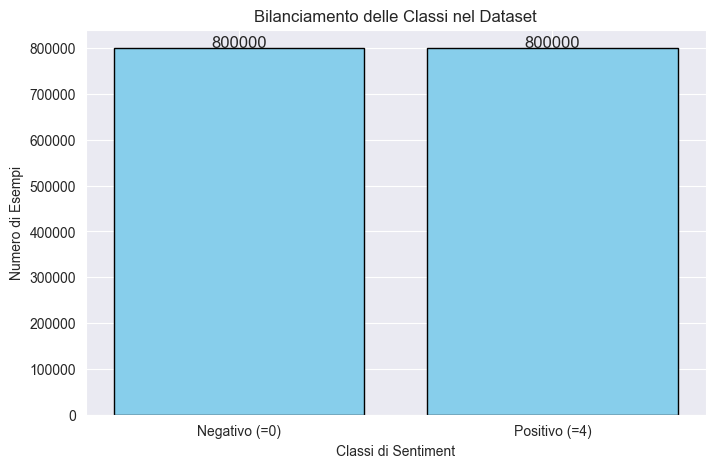
\includegraphics[width=0.75\linewidth]{immagini/bilanciamento_sentiment140_raw.png}
    \caption{Bilanciamento delle Classi nel Dataset completo Sentiment140}
    \label{fig:enter-label}
\end{figure}
\subsection{Analisi esplorativa del dataset ridotto}
Per ridurre il dataset mantenendo l’equilibrio tra le classi, è stato applicato un \textbf{campionamento stratificato}. In questo modo, la proporzione di tweet positivi e negativi nel sottoinsieme rispecchia quella del dataset originale.\\Per ottenere un campione di 100.000 tweet dai 1.600.000 iniziali è stata utilizzata una frazione di 0.0625 (100.000 / 1.600.000). Il campionamento, effettuato in modo stratificato rispetto alla variabile \textbf{target}, ha suddiviso il dataset in due strati corrispondenti alle classi di sentiment, prelevando casualmente un campione da ciascuno. Per garantire la riproducibilità, è stato impostato un seed fisso (random\_seed = 46).\\Il risultato è un dataset ridotto di 100.000 tweet, che mantiene una \textbf{distribuzione bilanciata} (50.000 tweet per ciascuna classe), come confermato dall’istogramma riportato di seguito.
\begin{figure}[H]
    \centering
    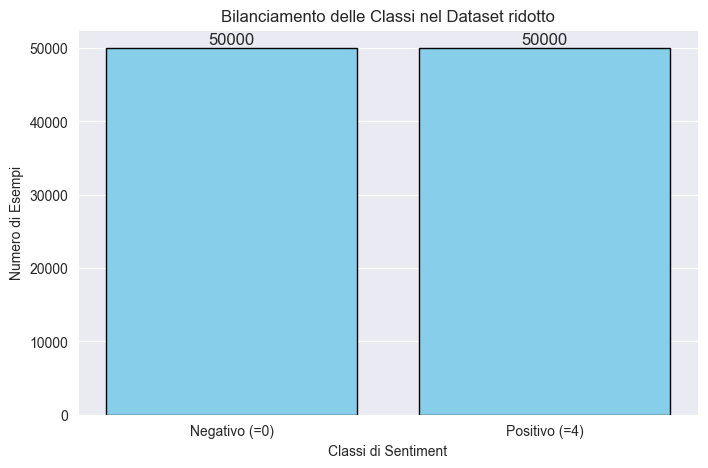
\includegraphics[width=0.75\linewidth]{immagini/bilanciamento_sentiment140_reduced.png}
    \caption{Bilanciamento delle Classi nel Dataset ridotto}
    \label{fig:enter-label}
\end{figure}
Analogamente al dataset originale, anche il sottoinsieme \textbf{non presenta valori nulli o stringhe vuote} e conserva le 6 caratteristiche iniziali, che saranno successivamente modificate nella fase di data preparation. \\Sono stati individuati 296 \textbf{tweet duplicati}, pari a circa lo 0,3\% del dataset.\\L’\textbf{analisi della lunghezza} dei tweet ha evidenziato una lunghezza media di 74,1 caratteri, con un minimo di 7 e un massimo di 243 caratteri. I \textbf{tweet con una lunghezza superiore a 140 caratteri} potrebbero essere il risultato di errori di scraping (considerando che nel 2009 il limite era di 140 caratteri)  come ad esempio il tweet nell'immagine di seguito: 
\begin{figure}[H]
    \centering
    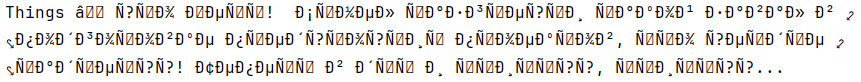
\includegraphics[width=0.75\linewidth]{immagini/tweet_lunghezza_max.png}
    \caption{Tweet di lunghezza massima, si possono notare errori di scraping }
    \label{fig:enter-label}
\end{figure}
Per questo motivo richiederanno un’attenzione particolare in fase di data preparation. \\Analogamente, i\textbf{ tweet con meno di 10 caratteri} saranno ulteriormente analizzati per valutare se il loro contenuto sia effettivamente significativo o se debbano essere esclusi dalla fase di modellazione. Nello specifico sono stati identificati 997 tweet con oltre 140 caratteri e 200 tweet con meno di 10 caratteri ma la maggior parte dei tweet si trova tra i 25 e i 75 caratteri come si può osservare nell'istogramma di seguito.
\begin{figure}[H]
     \centering
     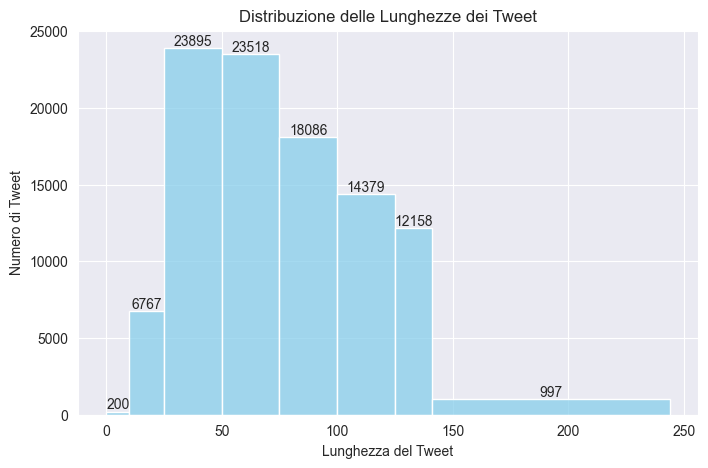
\includegraphics[width=0.75\linewidth]{immagini/lunghezza_tweet.png}
     \caption{Distribuzione delle lunghezze dei tweet}
     \label{fig:enter-label}
 \end{figure}
Tramite \textbf{Wordcloud} viene fornita una base visiva analizzare le parole più frequenti per ciascuna classe per fare un confronto e individuare anomalie o esigenze di pulizia dei dati:
 \begin{itemize}
     \item \textbf{Wordcloud sentiment negativo}: Dalla wordcloud relativa ai tweet negativi emergono parole dominanti come "work", "sorry", "tired", che riflettono chiaramente il contesto emotivo negativo. Tuttavia, è evidente anche la presenza di artefatti testuali non processati correttamente, come "amp", "u", "quot" e altri termini, che indicano la necessità di ulteriori interventi di pulizia dei dati. 
\begin{figure}[H]
    \centering
    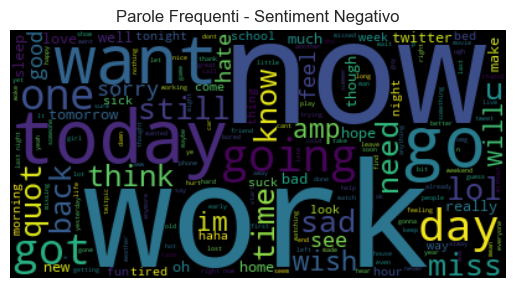
\includegraphics[width=0.75\linewidth]{immagini/understanding_wordclound_negativo.png}
  
    \label{fig:enter-label}
\end{figure}
 \end{itemize}
 \begin{itemize}
     \item \textbf{Wordcloud sentiment positivo}: Si possono notare le parole dominanti nel contesto positivo come "love", "thank", "good", "awesome" ecc... ma sono anche evidenti la grande quantità di artefatti di testo non processato correttamente come "amp", "u", "quot" e altri termini.
\begin{figure}[H]
    \centering
    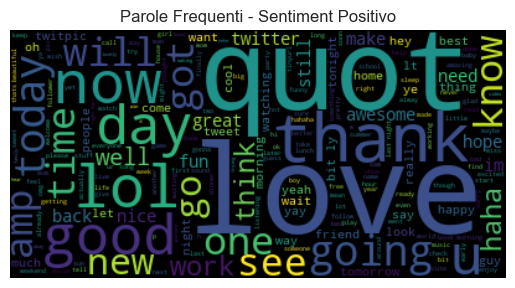
\includegraphics[width=0.75\linewidth]{immagini/understanding_wordcloud_positivo.png}
    \label{fig:enter-label}
\end{figure}
 \end{itemize}
\textbf{Parole condivise tra sentiment positivo e negativo}: Si nota che alcune parole, come "day" e "time", sono condivise tra i tweet positivi e negativi. Queste parole possono rappresentare una sfida per il modello di classificazione, poiché il loro significato varia in base al contesto. Saranno pertanto analizzate più approfonditamente nelle fasi successive del progetto.
\\Durante l'analisi preliminare, è stato calcolato il \textbf{n}\textbf{umero di tweet contenenti URL, menzioni (@username), hashtag (\#argomento) ed emoji testuali}. Per visualizzare meglio la distribuzione di queste caratteristiche, è stato creato un istogramma che riporta la frequenza relativa a ciascuna categoria. 
\begin{figure}[H]
    \centering
    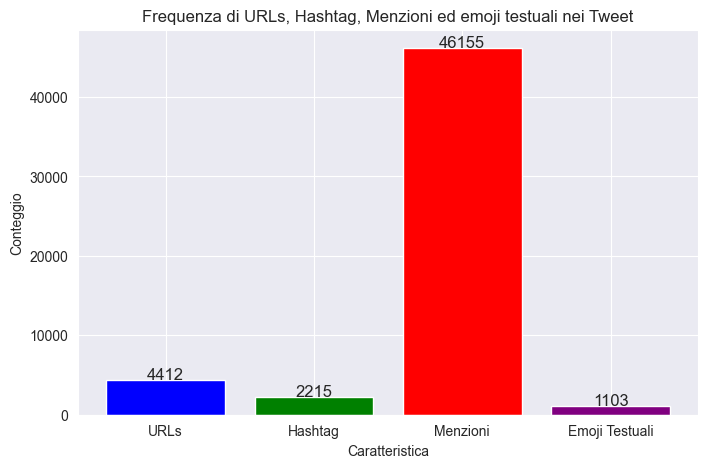
\includegraphics[width=0.75\linewidth]{immagini/frequenza_tweet_understanding.png}
    \label{fig:enter-label}
\end{figure}
Dall'istogramma emerge chiaramente che le menzioni (@username) sono la caratteristica più frequente, seguite da URL e hashtag, mentre la presenza di emoji testuali è significativamente più bassa. Questi risultati evidenziano l'importanza di trattare adeguatamente tali elementi durante la fase di data preparation, poiché possono influenzare il modello di sentiment analysis. 
\section{Identificazione delle variabili chiave e delle correlazioni}
Le variabili chiave individuate sono \textbf{"target"} e \textbf{"text"}. La variabile \textbf{"target"} rappresenta l’etichetta di sentiment, con valore \textbf{0} per i tweet negativi e \textbf{4} per quelli positivi, mentre \textbf{"text"} contiene il contenuto testuale da cui estrarre le informazioni utili per la classificazione. Sarà la variabile \textbf{"target"} quella che il classificatore dovrà predire sulla base delle caratteristiche estratte dal testo. La correlazione tra queste due variabili emerge dall’analisi della distribuzione delle parole: termini come \textit{"love"} e \textit{"thank"} compaiono frequentemente nei tweet positivi, mentre parole come \textit{"tired"} e \textit{"sorry"} sono più ricorrenti nei tweet negativi. Questa relazione tra il linguaggio utilizzato e il sentiment assegnato rappresenta il principio fondamentale su cui si basa l’addestramento del modello. 
\chapter{Data Preparation}
Anche questa fase è stata condotta con l'ausilio di Jupyter Notebook per \textbf{verificare in tempo reale gli effetti delle trasformazioni} e individuare eventuali problematiche nel testo.\\Durante la fase di data understanding si è osservato che nel dataset \textbf{non erano presenti valori nulli o stringhe vuote}, quindi non è stato necessario gestire questi aspetti durante la data preparation. \\Non sono state applicate tecniche di feature scaling a causa della natura dei modelli di classificazione e delle tecniche di rappresentazione testuale adottata:
\begin{itemize}
    \item \textbf{Per Naive Bayes:} Questo modello si basa su distribuzioni di frequenza e probabilità condizionate. Applicare uno scaling potrebbe alterare la distribuzione naturale delle feature, interferendo con la stima accurata delle probabilità e riducendo l’efficacia del modello.
    \item \textbf{Per la Logistic Regression:} La rappresentazione del testo mediante TF-IDF include già una normalizzazione intrinseca delle feature, rendendo superfluo un ulteriore scaling. Per la rappresentazione BoW(Bag Of Words), sebbene il feature scaling possa migliorare le performance, è stato scelto di mantenerla nella sua forma originale. Questo consente un confronto più diretto tra la Logistic Regression con BoW e Naive Bayes con BoW, mettendo in evidenza le differenze tra i due approcci. 
\end{itemize}
 \section{Pulizia preliminare del dataset}
 In questa fase sono state selezionate le feature essenziali, riformattati i valori del target, rimossi i duplicati e filtrati i tweet con lunghezze anomale, garantendo un dataset più pulito e adatto all’analisi. Al termine di questo processo il dataset risultante è stato salvato per sottoporlo all'addestramento.
\subsection{ Feature selection}
Come già evidenziato nella fase di data understanding, le feature principali individuate nel dataset sono text (testo del tweet) e target (sentiment del tweet, inizialmente codificato come 0 = negativo e 4 = positivo). Essendo queste le caratteristiche più rilevanti per il problema in esame, tutte le altre feature sono state rimosse dal dataset.
\subsection{Modifica del target}
Per rendere più chiara e intuitiva l'interpretazione dei risultati, i valori del target sono stati convertiti in una codifica binaria standard: 0 per i tweet negativi e 1 per quelli positivi. Sebbene questa trasformazione non fosse strettamente necessaria, è stata adottata per allinearsi a una convenzione più diffusa e facilmente comprensibile. 
\subsection{Rimozione dei duplicati}
I 296 duplicati individuati nella fase di data understanding sono stati rimossi eliminando le copie ridondanti, mantenendo un'unica occorrenza per ciascun tweet.
\subsection{Filtraggio dei testi in base alla lunghezza}
Durante la fase di data understanding sono emersi testi con lunghezze anomale:
\begin{itemize}
    \item \textbf{Testi con più di 140 caratteri}: Probabilmente derivanti da errori di scraping, sono stati rimossi.
    \item \textbf{Testi con meno di 10 caratteri}: La maggior parte di questi conserva un significato utile per l'analisi del sentiment. Tuttavia, 18 tweet contenevano solo una menzione, senza apportare informazioni rilevanti, e sono stati eliminati.
\end{itemize}
\subsection{Dataset al termine della pulizia preliminare}
Nonostante la rimozione di alcune occorrenze, il dataset rimane comunque bilanciato con 49370 tweet di sentiment negativo e 49321 tweet di sentiment positivo:
\begin{figure}[H]
    \centering
    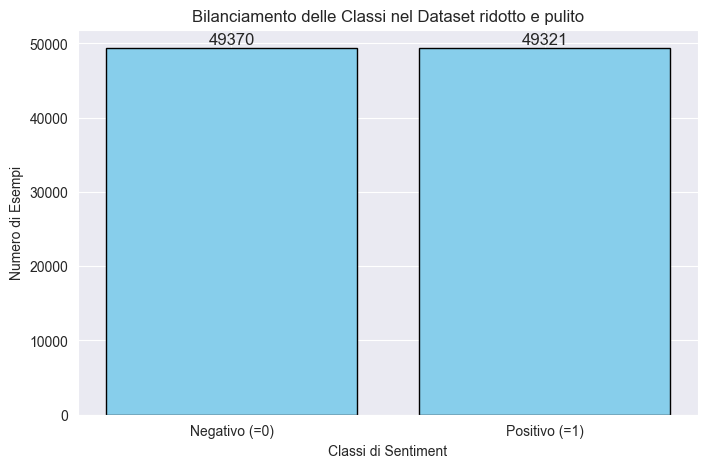
\includegraphics[width=0.75\linewidth]{immagini/bilanciamento_sentiment140_clean.png}
    \caption{Bilanciamento delle Classi nel Dataset dopo la pulizia preliminare}
    \label{fig:enter-label}
\end{figure}
\section{Pulizia del linguaggio naturale (NLP)}
Il linguaggio naturale attraverso vari passaggi viene ripulito per rimuovere rumore e informazioni non rilevanti in modo da estrarre informazioni significative per essere utilizzato efficacemente dai modelli di classificazione.  Sono stati individuate diverse operazioni da svolgere:
\begin{itemize}
    \item \textbf{Conversione del testo in minuscolo}: Questa trasformazione uniforma il testo eliminando le differenze tra lettere maiuscole e minuscole, in modo che parole identiche, ma con formattazioni diverse (es. 'Happy' e 'happy'), vengano trattate come uguali.
    \item \textbf{Rimozione degli URL}: Gli URL vengono rimossi perché non forniscono informazioni utili per l'analisi del sentiment e potrebbero introdurre rumore nel testo.
    \item \textbf{Rimozione delle menzioni}: Le menzioni vengono rimosse perché non influenzano direttamente il sentiment del tweet e potrebbero introdurre rumore nel testo.
    \item \textbf{Rimozione/Sostituzione delle entità html}: Le entità HTML come \texttt{\&amp;}, \texttt{\&quot;}, \texttt{\&lt;} e \texttt{\&gt;} sono state raccolte durante lo scraping dei tweet e la loro rimozione aiuta a ridurre il rumore nel testo. L'entità \texttt{\&apos;}, invece, è stata convertita in un apostrofo poiché rappresenta il corrispondente carattere testuale. Questo è stato mantenuto perché gli apostrofi possono essere utili per riconoscere abbreviazioni e contrazioni.
    \item \textbf{Sostituzione delle emoji testuali}: Le emoji possono fornire informazioni utili per la rilevazione del sentiment, quindi vengono sostituite con parole che ne rappresentano il significato. .
    \item \textbf{Rimozione degli hashtag}: viene eliminato solo il simbolo \verb|#|, mantenendo la parola associata, poiché potrebbe contenere informazioni utili per l'analisi del sentiment. 
    \item  \textbf{Espansione delle abbreviazioni}: Nei social sono utilizzate molte abbreviazioni e per questo motivo è stato creato un dizionario per espandere le abbreviazioni che sono utilizzate più spesso.
    \item \textbf{Espansione delle contrazioni}: L'inglese è un linguaggio ricco di contrazioni, si è deciso di espanderle per fare in modo che, all'interno del modello, una contrazione e la relativa espansione abbiano lo stesso significato.
    \item \textbf{Rimozione di punteggiatura e caratteri speciali}: I caratteri speciali sono stati rimossi poiché molto spesso sono dati da problemi durante lo scraping. Anche gli apostrofi rimanenti sono stati rimossi, in quanto, dopo l’espansione delle contrazioni e delle abbreviazioni, non apportano ulteriore significato. La punteggiatura rimanente è stata eliminata perché, sebbene possa in alcuni casi essere utile per interpretare il sentiment, soprattutto nel caso del Naive Bayes tende ad introdurre rumore. 
    \item  \textbf{Correzione Ortografica}: I tweet (così come altri post social) contengono numerosi errori di scrittura. Per ridurre il rumore, è stata applicata una correzione ortografica parola per parola. 
    \item \textbf{Normalizzazione degli spazi}: Molte frasi contengono spazi multipli o spazi alla fine della stringa che potrebbero introdurre rumore, per questo motivo sono stati rimossi.
    \item \textbf{Tokenizzazione}: La tokenizzazione è stata applicata per suddividere il testo in unità più piccole, dette token, facilitando l’applicazione di ulteriori processi come la lemmatizzazione e la rimozione di stopword
    \item \textbf{Lemmatizzazione}: Viene applicata per ridurre le parole alla loro forma base. È stata preferita allo stemming (che taglia semplicemente le desinenze) poiché utilizza un dizionario linguistico per ottenere la forma corretta della parola, contribuendo così a ridurre il numero di feature e a migliorare la generalizzazione del modello. 
    \item \textbf{Rimozione delle stopword}: Vengono rimosse perché sono parole comuni che non aggiungono valore informativo al testo, riducendo il rumore e migliorando le performance. 
    \item \textbf{Ricostruzione del testo}: Il testo viene ricostruito perché il vettorizzatore BoW lavora su stringhe di testo complete e non su liste di token. Ricostruendo il testo, si garantisce che la fase di feature extraction possa avvenire correttamente 
\end{itemize}
A questo punto sono state analizzate le wordcloud per verificare l'efficacia della pulizia:
\begin{figure}[H]
    \centering
    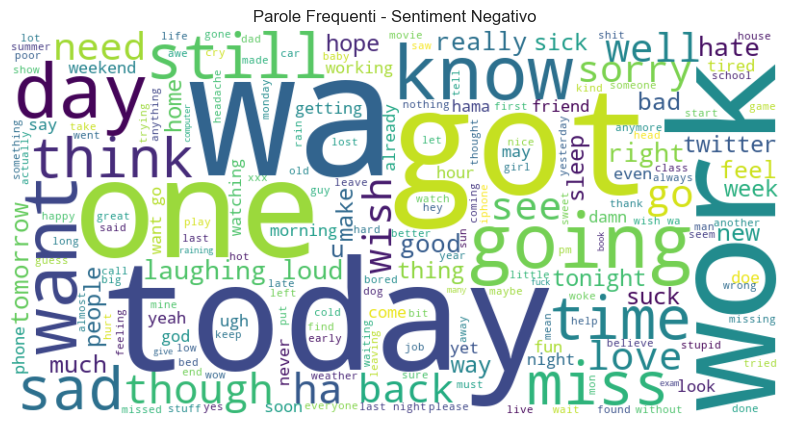
\includegraphics[width=0.75\linewidth]{immagini/wordcloud_negativo_conwa.png}
\end{figure}
\begin{figure}[H]
    \centering
    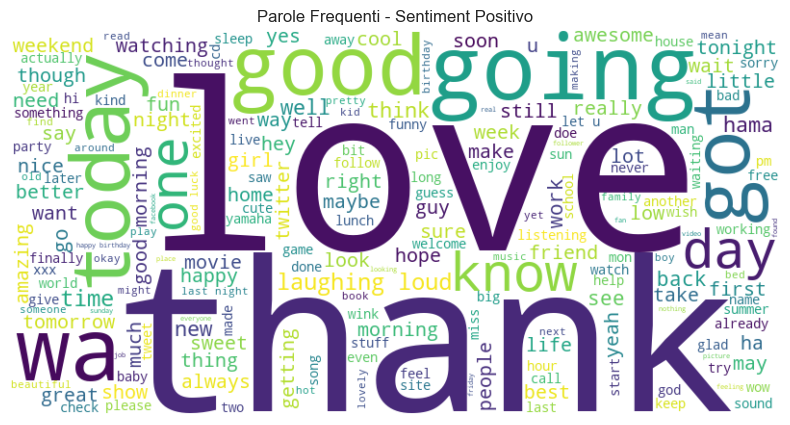
\includegraphics[width=0.75\linewidth]{immagini/wordcloud_positivo_conwa.png}
    \label{fig:enter-label}
\end{figure}
Si puo notare che grazie alla pulizia parole come \texttt{amp}, \texttt{u},  \texttt{quot} e molte altre che creavano rumore non sono più presenti. È  emersa  la parola "wa" che compare sia nei tweet negativi che quelli positivi. Poiché potrebbe essere un’abbreviazione di più termini e, in generale, non aggiunge informazioni rilevanti per l’analisi del sentiment, si è deciso di rimuoverla. Dopo la rimozione, sono state generate nuove wordcloud per confermare l’efficacia della pulizia:
\begin{figure}[H]
    \centering
    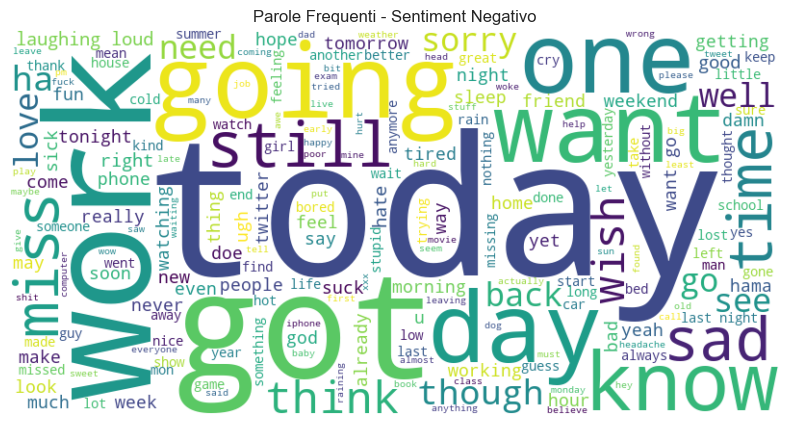
\includegraphics[width=0.75\linewidth]{immagini/wordcloud_negativo_nowa.png}
    \label{fig:enter-label}
\end{figure}
\begin{figure}[H]
    \centering
    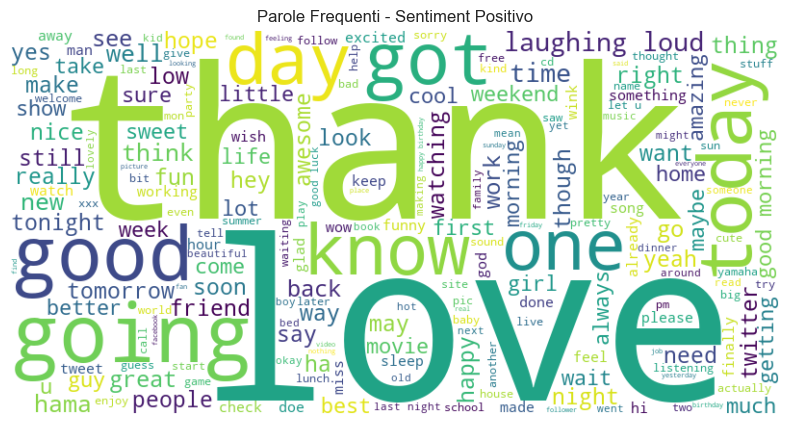
\includegraphics[width=0.75\linewidth]{immagini/wordcloud_positivo_nowa.png}

    \label{fig:enter-label}
\end{figure}
A questo punto si può continuare con la feature extraction poichè i dati sono stati ripuliti.
\section{Feature extraction}
Durante la fase di feature extraction, il processo di trasformazione dei tweet in vettori numerici è stato implementato utilizzando due \textbf{tecniche di rappresentazione testuale} che saranno successivamente messe a confronto: \textbf{Bag of Words (BoW)} e \textbf{TF-IDF}.
\begin{itemize}
    \item \textbf{Bag of Words (BoW):} Con il metodo BoW, ogni tweet viene convertito in un vettore in cui ogni posizione rappresenta una parola e il valore corrisponde al numero di volte in cui quella parola compare nel tweet. Questo approccio è molto diretto e, soprattutto, utile nei casi in cui parole frequenti  (pur essendo comuni) possono essere indicative del sentiment espresso. 
    \item \textbf{TF-IDF:} Invece di limitarsi a contare le occorrenze, il metodo TF-IDF valuta l'importanza di ogni parola all'interno dell'intero insieme di tweet. L'idea è di ridurre l'impatto delle parole che compaiono troppo frequentemente e che, di solito, non forniscono informazioni particolarmente distintive, dando maggiore rilevanza a termini meno comuni ma potenzialmente più significativi. Tuttavia, va detto che alcune parole molto frequenti possono comunque essere utili per capire il sentiment, e in questi casi il semplice conteggio del BoW può rivelarsi più efficace. 
\end{itemize}
 Per realizzare queste rappresentazioni sono stati utilizzati strumenti della libreria scikit-learn:
\begin{itemize}
    \item \textbf{CountVectorizer} per ottenere la rappresentazione BoW.
    \item \textbf{TfidfVectorizer} per calcolare i pesi TF-IDF.
\end{itemize}
Queste tecniche permettono di trasformare i tweet in dati numerici, rendendo possibile l'analisi del sentiment attraverso l'uso di modelli di machine learning. 
\section{\textbf{Conclusioni}}
 La fase di Data Preparation ha garantito un dataset di qualità per il modeling attraverso una serie di operazioni mirate alla pulizia e trasformazione del testo. Dopo una prima selezione delle feature e riformattazione del target, sono stati eliminati i duplicati e filtrati i tweet con lunghezze anomale. \\Il testo è stato pulito tramite la pulizia del linguaggio naturale per ridurre il numero. Infine, il testo è stato trasformato in una rappresentazione numerica tramite BoW e TF-IDF. Questa fase ha ridotto il rumore nei dati, migliorando la qualità dell’informazione testuale e rendendo più efficace la classificazione del sentiment. La operazioni di pulizia saranno integrate nella pipeline dei modello per garantire un processo standardizzato e riproducibile.

\chapter{Data Modeling}
In questa sezione viene effettuato l'addestramento dei modelli con gli algoritmi di classificazione binaria menzionati nel Capitolo 2: \textbf{Naive Bayes} e \textbf{Logistic Regression}. Poichè entrambi i modelli lavorano con dati numerici il linguaggio naturale sarà convertito in una rappresentazione numerica mediante due tecniche di rappresentazione testuale: \textbf{TF-IDF} e \textbf{Bag of Words}. Saranno quindi addestrate 4 configurazioni diverse:
\begin{itemize}
    \item \textbf{Naive Bayes con BoW}
    \item \textbf{Naive Bayes con TF-IDF }
    \item \textbf{Logistic Regression con BoW}
    \item \textbf{Logistic Regression con TF-IDF}
\end{itemize}
Per decidere quale delle 4 configurazione sarà ulteriormente validata e messa in funzione per classificare le frasi all'interno dell'interfaccia grafica,si procederà a una valutazione delle performance ottenute tramite \textbf{Stratified k-Fold Cross-Validation}. Questa tecnica suddivide i dati in k sottoinsiemi (\textbf{folds}). Il modello viene addestrato su k-1 fold e testato sul fold rimanente. Questo processo viene ripetuto k volte, usando ogni fold come test almeno una volta. Il campionamento stratificato garantisce che ogni fold rispecchi la distribuzione complessiva delle classi, ottenendo così dei fold bilanciati. In questo caso, si è deciso di utilizzare \textbf{k=10}.  \\Per valutare le prestazioni di ogni configurazione verranno calcolate le metriche di \textbf{accuracy}, \textbf{precision} e \textbf{recall} per ciascun fold, per poi effettuare una media sui valori ottenuti nelle 10 esecuzioni. In questo modo si otterranno tre metriche meno influenzate dalla specifica suddivisione iniziale del dataset. Infine, verrà selezionato il modello con le prestazioni migliori.
\section{Algoritmi utilizzati}
Essendo il problema da risolvere un problema di classificazione binario ci sono un gran numero di algoritmi da poter scegliere, ne sono stati scelti due: Naive Bayes e Logistic Regression. \\L’obiettivo è confrontare le loro performance nell'ambiente, valutando l’impatto delle tecniche di rappresentazione testuale (\textbf{Bag of Words} e \textbf{TF-IDF}) sui risultati ottenuti. La validazione di ciascuna configurazione sarà effettuata tramite \textbf{Stratified k-Fold Cross-Validation} (k=10), in modo da garantire una valutazione robusta e meno dipendente dalla particolare suddivisione del dataset.
\subsection{Naive Bayes}
Naive Bayes è un classificatore semplice e veloce, particolarmente efficace in fase di addestramento e inferenza grazie all’assunzione di indipendenza tra le feature. Pur non rispecchiando sempre la realtà del linguaggio naturale (parole stettamente correlate saranno considerate in modo indipendente), offre un buon punto di partenza per la sentiment analysis su dataset di dimensioni contenute. Nel progetto, l’utilizzo di Naive Bayes in combinazione con BoW e TF-IDF permette di valutare l’impatto di tale assunzione sulle performance del modello. \\In particolare, è stata impiegata l’implementazione \textbf{MultinomialNB} della libreria scikit-learn. \textbf{MultinomialNB }è una variante del classificatore Naive Bayes adatta a dati discreti, come il conteggio delle parole in testo. È spesso utilizzata per problemi di \textit{text classification}, come la \textit{sentiment analysis}, poiché assume che le feature seguano una distribuzione multinomiale. Questo significa che il modello calcola la probabilità di appartenenza a una classe basandosi sulla frequenza con cui le parole appaiono nei documenti. 
\subsection{Logistic Regression}
La Logistic Regression è un metodo di classificazione lineare adatto a problemi binari, in grado di modellare in modo flessibile le relazioni tra le feature. Utilizzando le rappresentazioni testuali BoW e TF-IDF, il modello stima la probabilità di appartenenza a ciascuna classe tramite la funzione logistica, traducendo il risultato in una decisione binaria (con soglia tipica di 0.5). Pur richiedendo tempi di addestramento leggermente superiori, offre una migliore gestione delle interazioni tra i termini, risultando particolarmente efficace per l’analisi del sentiment nei tweet. \\Per la realizzazione del modello, è stata utilizzata l’implementazione \textbf{LogisticRegression}. 
\section{Addestramento del modello}
Per fare l'addestramento delle 4 configurazioni elencate sopra, è stata creata una pipeline che segue 3 passaggi fondamentali:
\begin{enumerate}
    \item \textbf{Preprocessing del linguaggio naturale}:Il testo viene prima processato seguendo i passaggi definiti nella fase di Data Preparation.
    \item \textbf{Trasformazione} delle frasi in una rappresentazione numerica: Il testo pulito viene trasformato in una rappresentazione numerica utilizzando una delle due tecniche: 
    \begin{itemize}
        \item \textbf{Bag of Words (BoW)}:Viene creato un dizionario che associa a ciascuna parola un indice univoco. Ogni frase viene convertita in un vettore in cui ogni cella rappresenta il numero di volte in cui la corrispondente parola del dizionario compare nella frase. In questo modo si costruisce una matrice in cui le righe rappresentano le frasi e le colonne i termini del dizionario. 
        \item \textbf{TF-IDF}: Anch'esso costruisce un dizionario e crea vettori allo stesso modo di BoW ma i conteggi contenuti in ogni cella vengono trasformati in pesi tramite il calcolo del TF-IDF \textbf{(Term Frequency-Inverse Document Frequency)}. In questo modo il peso di ogni parola aumenta se il termine è frequente in una specifica frase, ma diminuisce se è comune in tutto il dataset. Questo approccio enfatizza le parole più distintive per ciascun testo. 
    \end{itemize}
    \item \textbf{Applicazione del classificatore}: Una volta ottenuta la rappresentazione numerica, il classificatore (Naive Bayes o Logistic Regression, a seconda della configurazione scelta) viene addestrato sulla matrice risultante. Il modello impara così a correlare le caratteristiche numeriche del testo con la variabile target contenente il sentiment. 
\end{enumerate}
Durante la fase di \textbf{fit (addestramento)}:
\begin{enumerate}
    \item Il \textbf{testo viene processato} con i passaggi specificati nella fase di data preparation.
    \item Viene costruita la rappresentazione numerica (BoW o TF-IDF) e viene creato il dizionario. 
    \item Il classificatore viene addestrato sui vettori numerici e le etichette associate. 
\end{enumerate}
Durante la fase di\textbf{ predict} (predizione della caratteristica target):
\begin{enumerate}
    \item Il \textbf{testo viene processato} con i passaggi specificati nella fase di data preparation.
    \item I testi puliti vengono \textbf{trasformati in vettori numerici} tramite (TF-IDF o BoW) utilizzando il dizionario già appreso durante la fase di fit. 
    \item Il classificatore utilizza ciò che ha imparato durante la fase di fit per effettuare la \textbf{previsione del sentiment}.
\end{enumerate}
Per valutare le prestazioni del modello in modo robusto, viene utilizzata la  \textbf{Stratified k-Fold Cross-Validation} che divide il dataset in 10 fold. Per ciascun fold, 9 parti vengono usate per addestrare la pipeline (fase di fit) e la restante per valutarne le prestazioni (fase di predict). Le metriche (accuracy, precision, recall) calcolate in ogni fold vengono poi mediate per ottenere una stima complessiva più affidabile delle prestazioni del modello. 
\section{Confronto delle performance tramite metriche di valutazione}
Per decidere quale delle quattro configurazioni  verrà ulteriormente valutata e usata come base per una semplice interfaccia grafica di valutazione del sentiment, si confrontano le prestazioni in termini di precision, recall e accuracy. Queste metriche vengono calcolate sia tramite la stratified k-Fold cross-validation (a 10 fold) e sia su un piccolo dataset composto da 1200 tweet in inglese (contenenti errori di battitura, slang, abbreviazioni, caratteri speciali, menzioni emoji testuali e hashtag) che è stato generato mediante l'utilizzo dell'LLM OpenAI o3-mini. La configurazione che ottiene i risultati complessivi migliori (cioè quella che riesce a garantire le metriche più elevate) sarà quella selezionata per i passaggi successivi. 
Durante la fase di trasformazione del testo, vengono utilizzati due parametri fondamentali per filtrare il vocabolario: \textbf{min\_df} e \textbf{max\_df}. Questi sono impostabili sia in CountVectorizer che in TfidfVectorizer e servono a filtrare il vocabolario durante la trasformazione del testo in una rappresentazione numerica. In particolare: 
\begin{itemize}
    \item \textbf{min\_df} indica il numero minimo di frasi in cui un termine deve comparire per essere incluso nel dizionario. Con questo parametro si escludono i termini troppo rari che potrebbero introdurre rumore nella rappresentazione.
    \item  \textbf{max\_df} indica la proporzione massima di documenti oltre la quale un termine viene considerato troppo comune e quindi non discriminante. Questo aiuta a eliminare i termini generici che compaiono in quasi tutti i documenti, riducendo così l’impatto di parole non informative.
\end{itemize}
Nel progetto è stata impostata per tutte le configurazioni \textbf{min\_df = 5} (una parola viene considerata nel vocabolario solo se appare in almeno 5 frase) e \textbf{max\_df = 0.9} (parole che compaiono in oltre il 90\% delle frasi non vengono considerate perchè troppo frequenti). Per le configurazioni che si dimostreranno più promettenti, si prevede di sperimentare con diversi valori di min\_df e max\_df, al fine di ottimizzare ulteriormente le prestazioni del modello. 
\subsection{Performance Naive Bayes con BoW}
\begin{figure}[H]
    \centering
    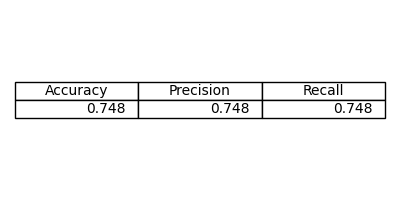
\includegraphics[width=0.75\linewidth]{immagini_modeling/nb_bow.png}
    \caption{Performance medie sui fold}
    \label{fig:enter-label}
\end{figure}
\begin{figure}[H]
    \centering
    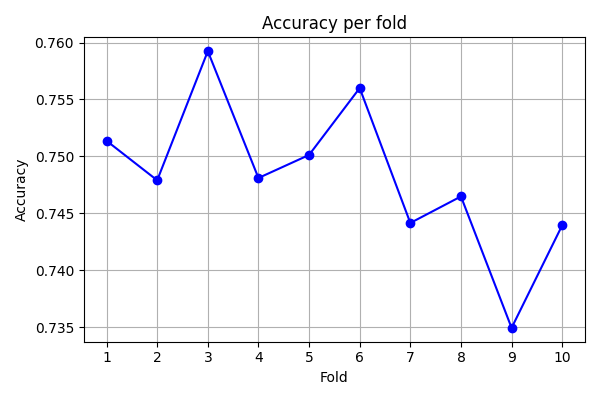
\includegraphics[width=0.75\linewidth]{immagini_modeling/accuracy_nb.png}
    \label{fig:enter-label}
\end{figure}
\begin{figure}[H]
    \centering
    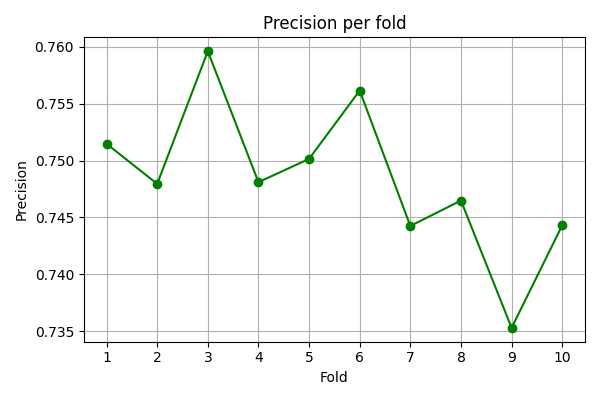
\includegraphics[width=0.75\linewidth]{immagini_modeling/precision_nb.png}
   
    \label{fig:enter-label}
\end{figure}
\begin{figure}[H]
    \centering
    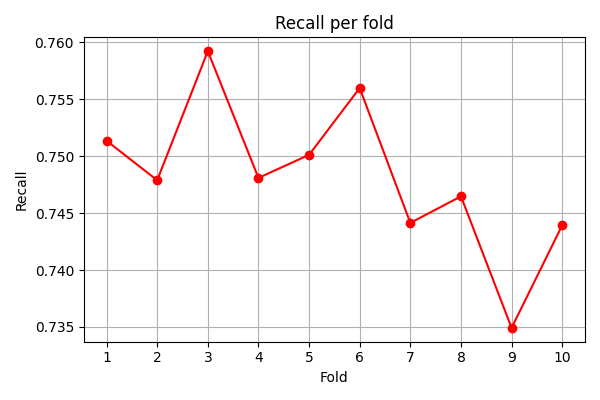
\includegraphics[width=0.75\linewidth]{immagini_modeling/recall_nb.png}
    \label{fig:enter-label}
\end{figure}
\subsubsection{Performance su dataset LLM}
\begin{figure}[H]
    \centering
    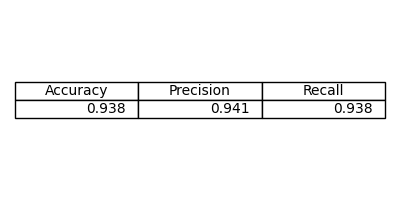
\includegraphics[width=0.75\linewidth]{immagini_modeling/nb_llm.png}
    \caption{Performance su dataset LLM}
    \label{fig:enter-label}
\end{figure}
\begin{figure}[H]
    \centering
    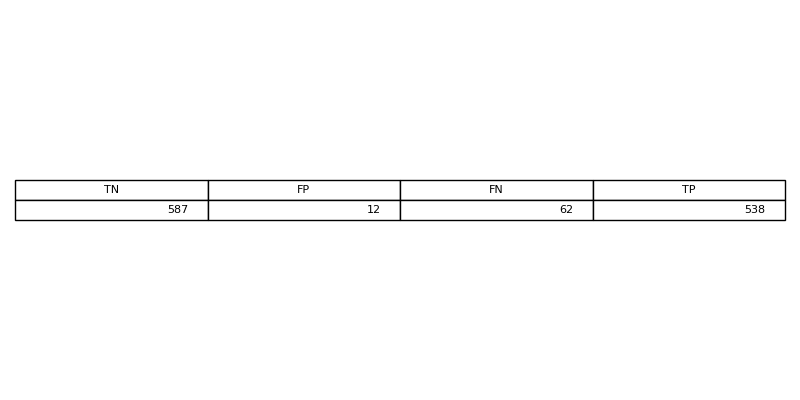
\includegraphics[width=1\linewidth]{immagini_modeling/nb_matrice.png}
    \caption{Matrice di confusione}
    \label{fig:enter-label}
\end{figure}
\subsection{Performance Naive Bayes con TF\_IDF}
\begin{figure}[H]
    \centering
    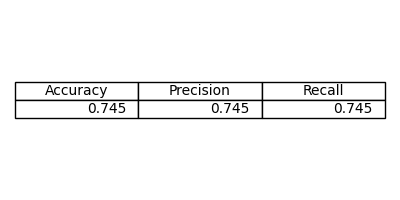
\includegraphics[width=0.75\linewidth]{immagini_modeling/nb_tfidf.png}
    \caption{Performance medie sui fold}
    \label{fig:enter-label}
\end{figure}
\begin{figure}[H]
    \centering
    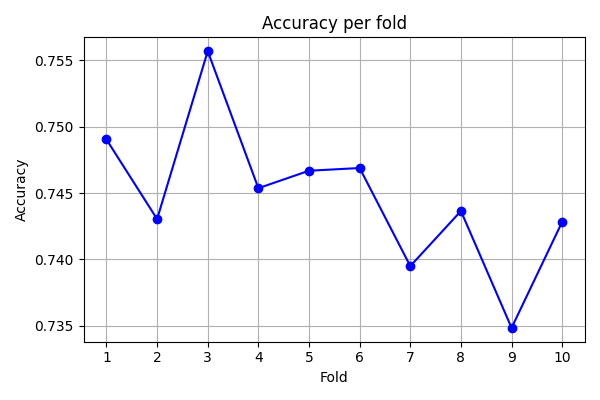
\includegraphics[width=0.75\linewidth]{immagini_modeling/accuracy_nb_tfidf.png}
    \label{fig:enter-label}
\end{figure}
\begin{figure}[H]
    \centering
    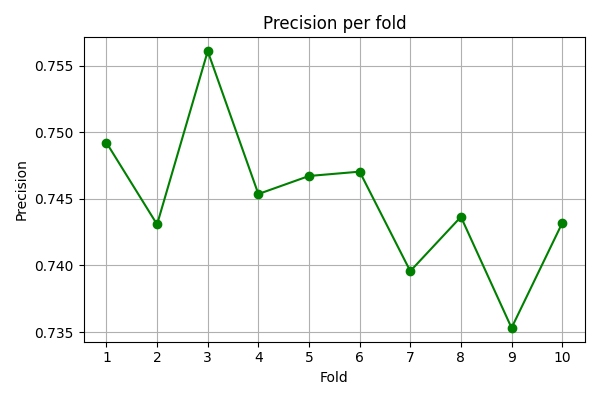
\includegraphics[width=0.75\linewidth]{immagini_modeling/precision_nb_tfidf.png}
    \label{fig:enter-label}
\end{figure}

\begin{figure}[H]
    \centering
    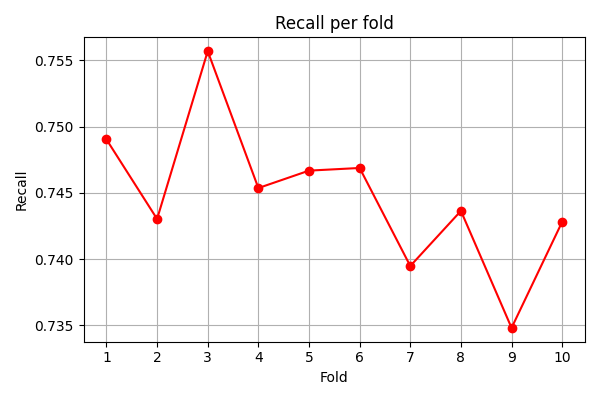
\includegraphics[width=0.75\linewidth]{immagini_modeling/recall_nb_tfidf.png}
    \caption{Enter Caption}
    \label{fig:enter-label}
\end{figure}
\subsubsection{Performance su dataset LLM}
\begin{figure}[H]
    \centering
    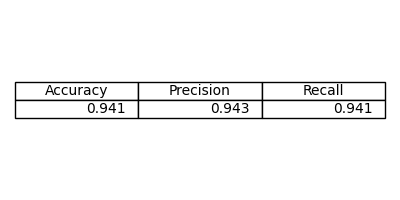
\includegraphics[width=0.75\linewidth]{immagini_modeling/nb_tfidf_llm.png}
    \caption{Performance su dataset LLM}
    \label{fig:enter-label}
\end{figure}
\begin{figure}[H]
    \centering
    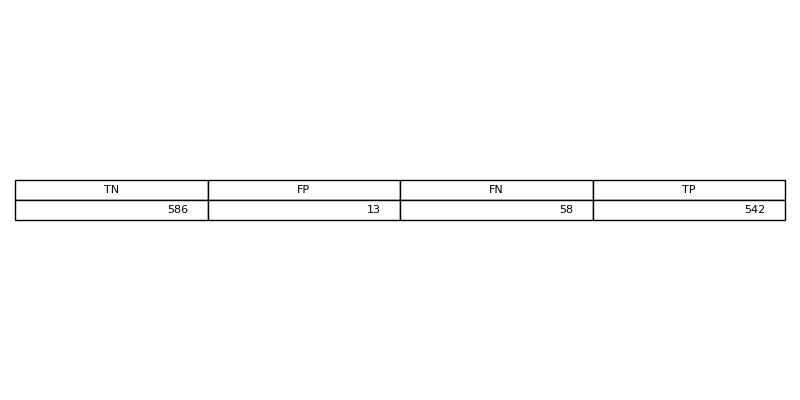
\includegraphics[width=1\linewidth]{immagini_modeling/matrice_nb_tfidf.png}
    \caption{Matrice di confusione}
  
    \label{fig:enter-label}
\end{figure}
\subsection{Performance Logistic Regression con BoW}
\begin{figure}[H]
    \centering
    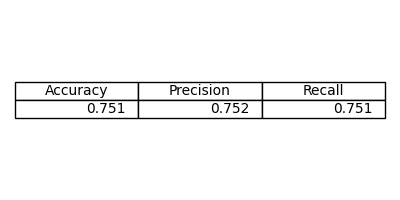
\includegraphics[width=0.75\linewidth]{immagini_modeling/lr.png}
    \caption{Performance medie sui fold}
    \label{fig:enter-label}
\end{figure}
\begin{figure}[H]
    \centering
    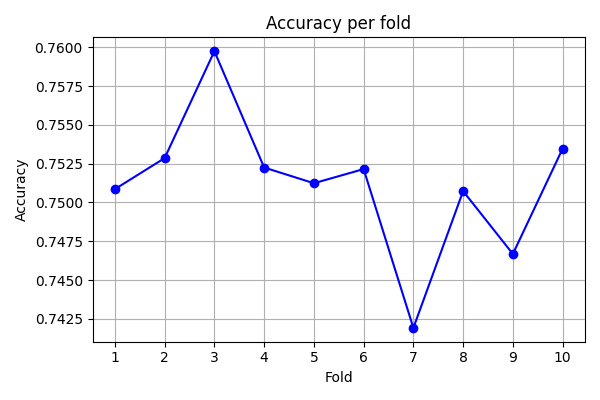
\includegraphics[width=0.75\linewidth]{immagini_modeling/lr_accuracy.png}
    \label{fig:enter-label}
\end{figure}
\begin{figure}[H]
    \centering
    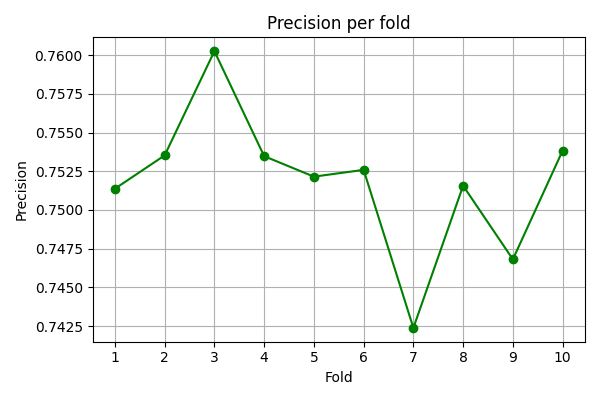
\includegraphics[width=0.75\linewidth]{immagini_modeling/lr_precision.png}
    
    \label{fig:enter-label}
\end{figure}
\begin{figure}[H]
    \centering
    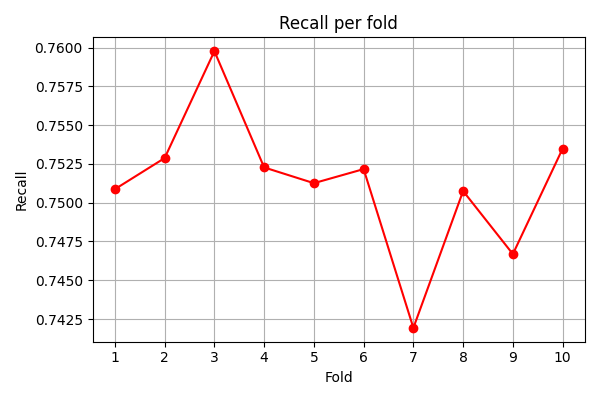
\includegraphics[width=0.75\linewidth]{immagini_modeling/recall_lr.png}
    \label{fig:enter-label}
\end{figure}
\subsubsection{Performance su dataset LLM}
\begin{figure}[H]
    \centering
    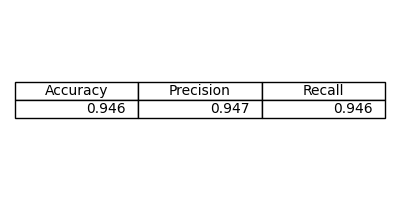
\includegraphics[width=0.75\linewidth]{immagini_modeling/lr_performance.png}
    \caption{Performance su dataset LLM}
    \label{fig:enter-label}
\end{figure}
\begin{figure}[H]
    \centering
    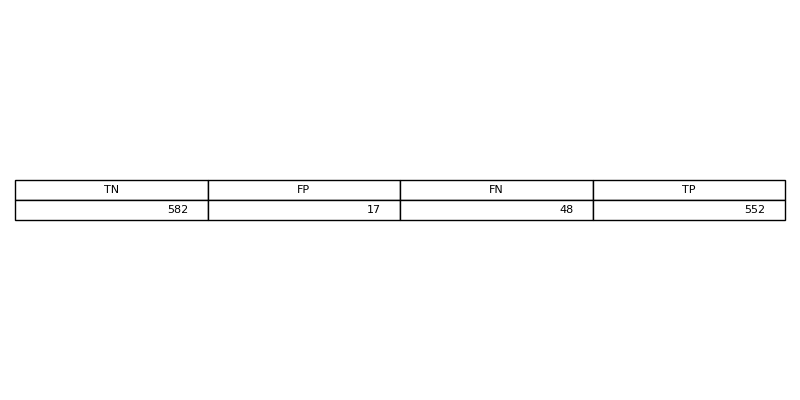
\includegraphics[width=1\linewidth]{immagini_modeling/matrice_lr.png}
    \caption{Matrice di confusione}
    \label{fig:enter-label}
\end{figure}
\subsection{Performance Logistic Regression con TF-IDF}
\begin{figure}[H]
    \centering
    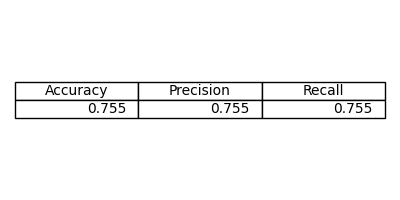
\includegraphics[width=0.75\linewidth]{immagini_modeling/lr_tfidf.png}
    \caption{Performance medie sui fold}
    \label{fig:enter-label}
\end{figure}
\begin{figure}[H]
    \centering
    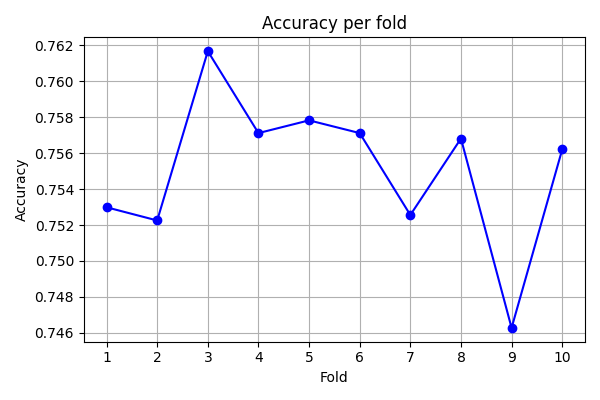
\includegraphics[width=0.75\linewidth]{immagini_modeling/accuracy_lr_tfidf.png}
    
    \label{fig:enter-label}
\end{figure}
\begin{figure}[H]
    \centering
    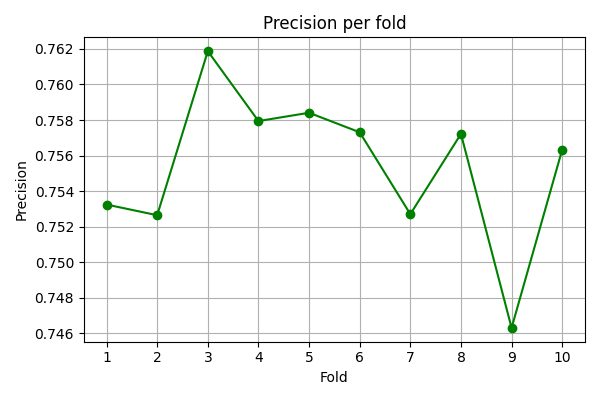
\includegraphics[width=0.75\linewidth]{immagini_modeling/precision_lr_tfidf.png}
    
    \label{fig:enter-label}
\end{figure}
\begin{figure}[H]
    \centering
    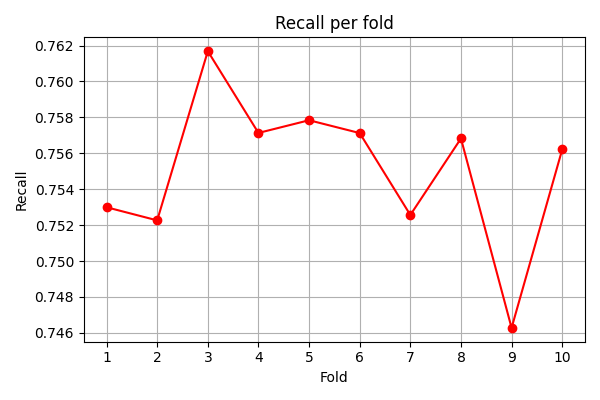
\includegraphics[width=0.75\linewidth]{immagini_modeling/recall_lr_tfidf.png}
    
    \label{fig:enter-label}
\end{figure}
\subsubsection{Performance su dataset LLM}
\begin{figure}[H]
    \centering
    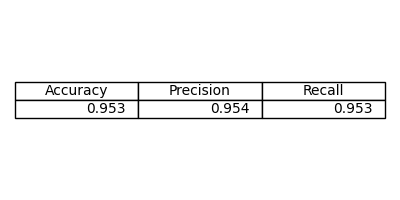
\includegraphics[width=0.75\linewidth]{immagini_modeling/lr_tfidf_llm.png}
    \caption{Performance su dataset LLM}
    \label{fig:enter-label}
\end{figure}
\begin{figure}[H]
    \centering
    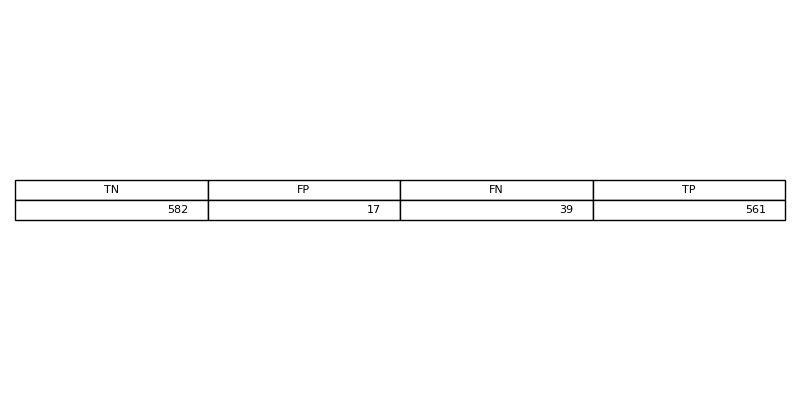
\includegraphics[width=1\linewidth]{immagini_modeling/matrice_tfidf_lr.png}
    \caption{Matrice di confusione}
    \label{fig:enter-label}
\end{figure}
\subsection{Modifica dei parametri min\_df e max\_df}
La combinazione con le migliori prestazioni in generale è quella di \textbf{Logistic Regression con TF-IDF}. Si è provato a fare dei ritocchi sui parametri min\_df e max\_df per provare a migliorare le prestazioni.
\begin{enumerate}
    \item  \textbf{min\_df = 1} e \textbf{max\_df=0.9}: Abbassando il parametro min\_df, durante la validazione con Stratified k-Fold Cross-Validation si è registrato un leggero aumento delle performance medie. Tuttavia, le performance sul dataset generato da LLM sono diminuite. Questo accade perché termini molto rari, presenti solo nel dataset di training, vengono appresi eccessivamente, dando meno importanza a termini più rilevanti per l’analisi del sentiment. Tale fenomeno porta a un leggero overfitting, perciò questo setting viene scartato.
    \begin{figure}[H]
        \centering
        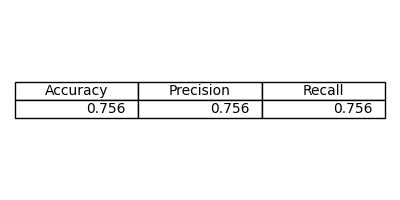
\includegraphics[width=0.75\linewidth]{immagini_modeling/parameter1.png}
        \caption{Performance medie sui fold}
        \label{fig:enter-label}
    \end{figure}
\begin{figure}[H]
    \centering
    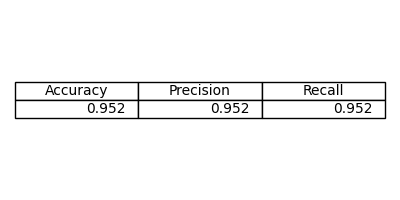
\includegraphics[width=0.75\linewidth]{immagini_modeling/parameter2.png}
    \caption{Performance su dataset LLM}
    \label{fig:enter-label}
\end{figure}
\item \textbf{min\_df = 10} e \textbf{max\_df = 0.9}: Alzando il parametro min\_df si è avuto un peggioramento generale delle performance. Questo è dovuto dal fatto che che alcune parole significative per l'analisi del sentiment vengono scartate. Il setting pertanto viene scartato.
\begin{figure}[H]
    \centering
    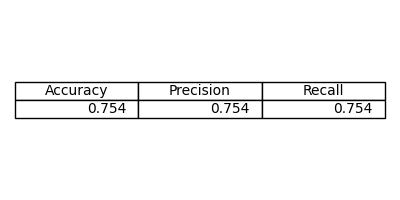
\includegraphics[width=0.75\linewidth]{immagini_modeling/parameter3.png}
    \caption{Performance medie sui fold}
    \label{fig:enter-label}
\end{figure}
\begin{figure}[H]
    \centering
    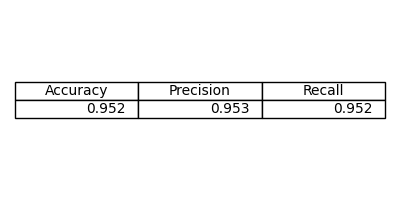
\includegraphics[width=0.75\linewidth]{immagini_modeling/parameter4.png}
    \caption{Performance su dataset LLM}
    \label{fig:enter-label}
\end{figure}
\item \textbf{min\_df = 5} e \textbf{max\_df=0.2}: Abbassando il parametro max\_df, si cerca di escludere le parole troppo frequenti, ma si è constatato un leggero peggioramento generale delle performance. La ragione è che la maggior parte delle parole poco significative era già stata rimossa durante la fase di data preparation, e un valore troppo basso di max\_df esclude anche termini utili per l’analisi del sentiment. Per questo motivo, anche questo setting viene scartato. 
\begin{figure}[H]
    \centering
    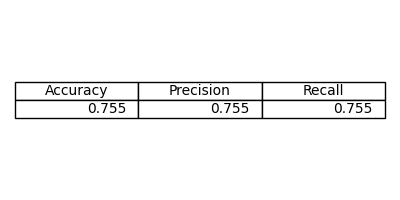
\includegraphics[width=0.75\linewidth]{immagini_modeling/parameter5.png}
    \caption{Performance medie sui fold}
    \label{fig:enter-label}
\end{figure}
\end{enumerate}
\begin{figure}[H]
    \centering
    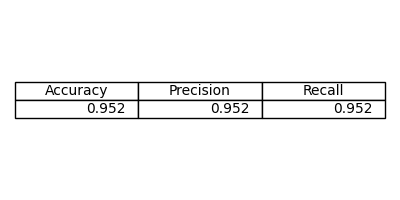
\includegraphics[width=0.75\linewidth]{immagini_modeling/parameter_6.png}
    \caption{Performance su dataset LLM}
    \label{fig:enter-label}
\end{figure}
I ritocchi sui parametri min\_df e max\_df hanno mostrato che sia impostazioni troppo permissive sia troppo restrittive possono influenzare negativamente le prestazioni del modello. L’impostazione ottimale rimane quella che trova un equilibrio tra la rimozione del rumore e la preservazione dei termini significativi per il sentiment. 
\section{Conclusioni}
Dall’analisi complessiva delle quattro configurazioni, è stato scelto il modello basato su \textbf{Logistic Regression con TF-IDF} (impostando min\_df = 5 e max\_df = 0.9). Questa configurazione ha offerto le migliori prestazioni complessive, sia in termini di accuracy, precision e recall, sia sul dataset generato dall’LLM. \\I grafici che mostrano le performance per fold (accuracy, precision e recall) contengono risultati poco variabili tra i vari fold grazie alla Stratified k-Fold Cross-Validation che garantisce che ogni fold sia un campione rappresentativo dell’intero dataset, mantenendo bilanciate le due classi all'interno del fold. \\Poiché il dataset è bilanciato, il \textbf{modello è in grado di trattare in modo equo entrambe le classi}, e ciò si riflette in metriche coerenti e simili. Grazie a questo fattore si sono ottenuti risultati comparabili in termini di accuracy, precision e recall. \\Il modello Logistic Regression con TF-IDF ha registrato \textbf{prestazioni migliori sul dataset generato dall’LLM} rispetto a quello utilizzato per l’addestramento valutato con la stratified k-fold. Questo miglioramento si può spiegare considerando che, sebbene il dataset LLM presenti un certo livello di rumore, esso non contiene tutti quegli elementi di rumore e ambiguità tipici del linguaggio dei social media, come slang estremamente variegato, abbreviazioni non standard ed errori di battitura sebbene sia stato richiesto al LLM di farlo utilizzando il prompt \textit{"Crea un dataset csv strutturato con 2 colonne: text e target, text deve contenere brevi tweet in inglese che devono contenere errori di battitura, slang, abbreviazioni, caratteri speciali, menzioni, emoji testuali e hashtag. Target deve contenere il sentiment del tweet che deve essere 1 per sentiment positivo e 0 per sentiment negativo. Il csv deve contenere 300 istanze." .}
\chapter{Evaluation}
In questa fase, il modello Logistic Regression con TF-IDF viene ulteriormente testato per verificare che le metriche di precision, recall e accuracy \textbf{soddisfino i valori minimi} definiti negli obiettivi di business. A tal fine, il modello è stato valutato sui 1.500.000 tweet rimanenti del dataset Sentiment140, che non sono stati utilizzati per il training, ottenendo i seguenti risultati.
\begin{figure}[H]
    \centering
    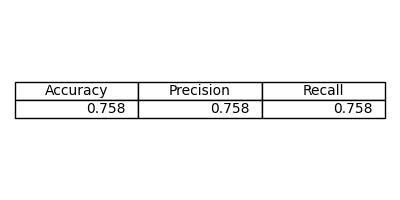
\includegraphics[width=0.75\linewidth]{immagini_modeling/performance_rim.png}
    \caption{Performance su dataset rimanente}
    \label{fig:enter-label}
\end{figure}
\begin{figure}[H]
    \centering
    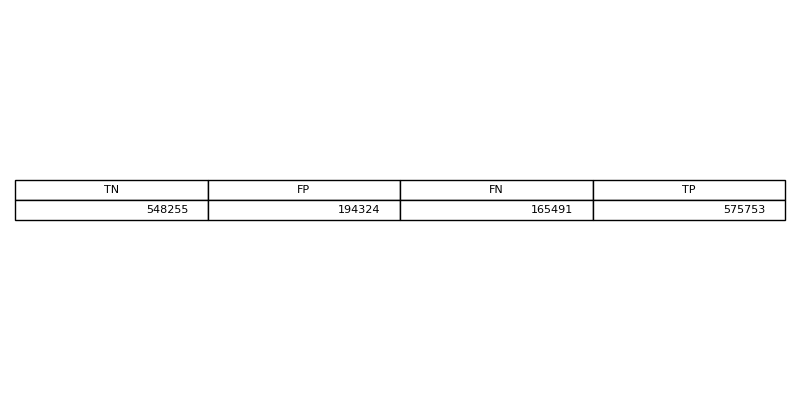
\includegraphics[width=1\linewidth]{immagini_modeling/matr_rimanente.png}
    \caption{Matrice di confusione su dataset rimanente}
    \label{fig:enter-label}
\end{figure}
I risultati sono ben superiori a quelli prefissati durante la definizione degli obiettivi. Si sono registrate addirittura prestazioni leggermente maggiori rispetto a quelle ottenute mediante Stratified k-Fold Cross-Validation nella fase precedente. \\Come si può notare Dalla matrice di confusione si evince che il modello mostra una leggera difficoltà nel classificare correttamente il sentiment negativo (il numero di falsi positivi è maggiore rispetto ai falsi negativi). Tuttavia, \textbf{il modello riesce a trattare in modo equo entrambe le classi}, garantendo una buona generalizzazione. \\ Il modello presenta \textbf{basso overfitting} per i seguenti motivi:
\begin{enumerate}
    \item Non si è registrata alcuna perdita di performance tra le valutazioni ottenute durante il modeling e quelle ottenute nella fase di evaluation. 
    \item Durante la fase di modeling si è notata una bassa differenza tra i vari fold.
    \item  Il modello ha registrato prestazioni significativamente superiori quando testato su un dataset generato da LLM, dimostrando la capacità di adattarsi a frasi provenienti da fonti e strutture diverse. 
\end{enumerate}
Il modello presenta \textbf{alcuni segni di underfitting} per i seguenti motivi:
\begin{enumerate}
    \item Pur ottenendo performance complessive con valori di precision, recall e accuracy attorno a 0.75, queste metriche indicano che il modello, pur funzionando in modo adeguato, non riesce a cogliere pienamente la complessità semantica insita in alcuni testi.
    \item Nei casi in cui le parole mostrano una forte correlazione contestuale, il modello tende a trattarle in maniera isolata, perdendo di vista il significato complessivo della frase.
    \item  L'osservazione mediante l'interfaccia creata durante la fase di deployment evidenzia situazioni critiche, come nella frase "What a good day to die", dove il sistema interpreta erroneamente il sentiment come positivo, segnale di una limitata capacità nel riconoscere sfumature linguistiche più sofisticate, come il sarcasmo.
\end{enumerate}
\chapter{Deployment}
In questa fase è stata realizzata una \textbf{semplice interfaccia} con tkinter che permette di inserire una frase di massimo 140 caratteri e tramite un pulsante effettuare la classificazione. Viene stampato "Sentiment negativo" o "Sentiment positivo" in base al sentiment rilevato e in caso di \textbf{basso livello di confidenza} (minore del 55\%) da parte del modello viene stampato un messaggio che segnala che la classificazione è incerta come ad esempio "Sentiment negativo (predizione incerta - Confidenza: 50.4\%)".\\Ecco alcuni esempi:
\begin{figure}[H]
    \centering
    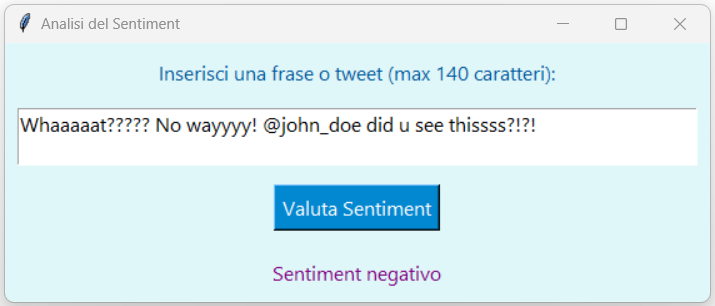
\includegraphics[width=0.75\linewidth]{immagini/sentimentnegativo.png}
    
    
\end{figure}
\begin{figure}[H]
    \centering
    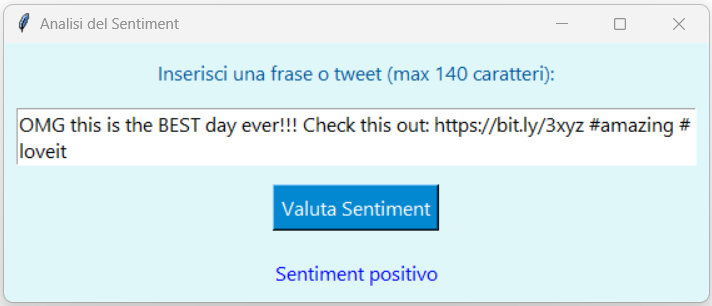
\includegraphics[width=0.75\linewidth]{immagini/sentimentpositivo.png}
    
    
\end{figure}
\begin{figure}[H]
    \centering
    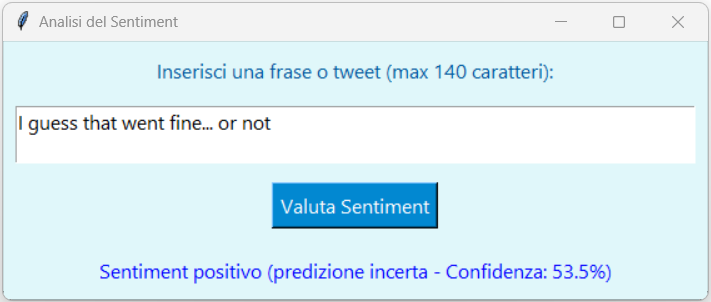
\includegraphics[width=0.75\linewidth]{immagini_modeling/incerta.png}
\end{figure}

\end{document}